\documentclass[11pt, conference, onecolumn]{IEEEtran}

% Packages for professional formatting
\usepackage[utf8]{inputenc}
\usepackage[T1]{fontenc}
\usepackage{cite}
\usepackage{amsmath,amssymb,amsfonts}
\usepackage{algorithmic}
\usepackage{graphicx}
\usepackage{textcomp}
\usepackage{xcolor}
\usepackage{booktabs}
\usepackage{float}
\usepackage{hyperref}

% Define colors for links
\definecolor{darkblue}{RGB}{0, 51, 102}
\hypersetup{colorlinks=true, linkcolor=darkblue, citecolor=darkblue, urlcolor=darkblue}

\begin{document}

% ==========================================
%                 COVER PAGE
% ==========================================
\begin{titlepage}
    \centering
    \vspace*{1.5in}
    
    {\Huge \bfseries Benchmarking DINO for Drone-View Object Detection on VisDrone\par}
    
    \vspace{1.5in}
    
    {\LARGE \textbf{CSE 429: Computer Vision and Pattern Recognition}\par}
    {\Large Final Project Report\par}
    
    \vspace{1.5in}
    
    {\large \textbf{Team Members:}\par}
    \vspace{0.2in}
    {\large 
    Jana Mohamed Elsalhy (120220093) \\
    Shiref Ashraf Mohamed (120220099) \\
    Ahmed Nagah Ramadan (120220116) \\
    Tasbih Othman Neamatallah (120220117) \\
    Karim Yaser Mazroua (120220118) \\
    Yasmeen Sameh Mohamed (120220143) \par}
    
    \vfill
    
    {\Large \textbf{Instructor:} Prof. Ahmed Gomaa\par}
    \vspace{0.3in}
    {\large May 8, 2026\par}
\end{titlepage}

% ==========================================
%           IEEE MAIN DOCUMENT
% ==========================================

\begin{abstract}
The rapid proliferation of Unmanned Aerial Vehicles (UAVs) has intensified the demand for robust, high-precision aerial object detection systems. However, standard convolutional and transformer-based architectures often struggle in the drone domain due to extreme scale variations, high object density, and severe background clutter. In this project, we implement and benchmark the state-of-the-art DINO (DETR with Improved DeNoising Anchor Boxes) model against the industry-standard YOLOv11 and a standard DETR baseline. Utilizing the VisDrone-DET2019 dataset, we evaluate the efficacy of Contrastive DeNoising (CDN) and anchor-free transformer logic in overcoming bipartite matching instability for small-scale targets. Due to the extreme computational requirements of training multi-scale transformers from scratch, our methodology focuses on a comparative review and evaluation of these models. Our experiments reveal the critical trade-offs between the end-to-end global reasoning of transformers and the high-speed inference of CNNs for edge deployment.
\end{abstract}

\begin{IEEEkeywords}
Object Detection, UAV, VisDrone, Transformers, DINO, YOLO, Edge Computing
\end{IEEEkeywords}

\section{Introduction}
Object detection from drone-mounted cameras is a critical enabling technology for applications including military surveillance, search and rescue operations, and autonomous traffic monitoring \cite{visdrone}. Despite advancements in computer vision, the UAV domain presents a unique set of non-trivial challenges that break standard detection paradigms. Aerial imagery suffers from extreme scale variance, perspective shifts, and high instance density, causing traditional bounding box algorithms to merge distinct entities.

Historically, models like YOLO and Faster R-CNN have dominated this space. However, the introduction of DETR (DEtection TRansformer) offered an end-to-end alternative. In this report, we explore \textbf{DINO}, a model that refines the DETR architecture through denoising mechanisms, to determine if its theoretical advantages translate to tangible performance gains on the challenging VisDrone dataset, comparing it directly with YOLOv11 and standard DETR variants.

\section{Scholarly Review \& Related Work}
Our approach is grounded in the rapid evolution of object detection paradigms. The transition from pure convolutional networks to refined transformer architectures represents a sequence of breakthroughs aimed at eliminating hand-crafted priors.

\subsection{The Evolution of Detection Architectures}

\subsubsection{CNN-Based Detectors}
Convolutional Neural Networks (CNNs), particularly the YOLO (You Only Look Once) family \cite{yolo_orig}, revolutionized real-time detection by framing the task as a single regression problem. Using anchor boxes, CNNs achieved remarkable speed. However, their reliance on dense anchor placement and Non-Maximum Suppression (NMS) creates bottlenecks in extremely crowded scenes, such as those found in drone imagery, where NMS often suppresses valid overlapping targets.

\begin{figure}[H]
    \centering
    % Placeholder for CNN Architecture Figure
    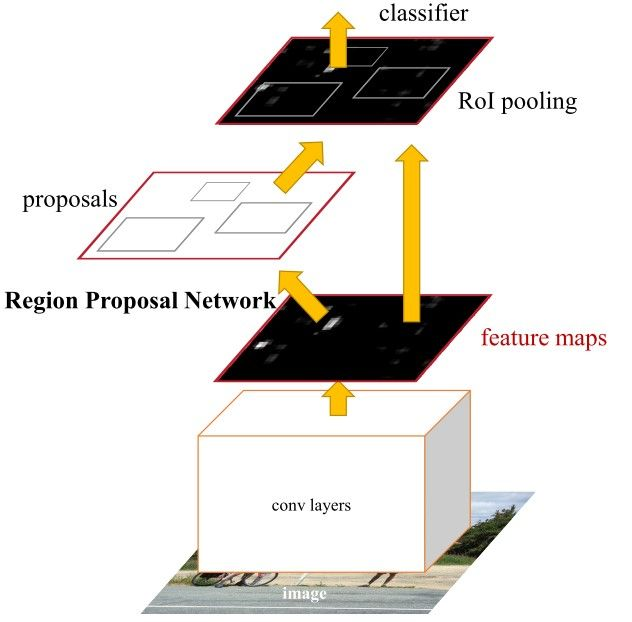
\includegraphics[width=0.6\linewidth]{figures/fr-cnn.png}
    \caption{Typical CNN-based Object Detection Pipeline (e.g., YOLO/Faster R-CNN) highlighting anchor boxes and NMS post-processing.}
    \label{fig:cnn}
\end{figure}

\subsubsection{DETR (DEtection TRansformer)}
To solve the NMS bottleneck, Carion et al. introduced DETR \cite{detr}. DETR treats object detection as a direct set prediction problem. By leveraging a global transformer architecture and bipartite matching (via the Hungarian algorithm), it completely eliminates the need for anchor boxes and NMS. However, standard DETR suffers from incredibly slow convergence (often requiring 500+ epochs) and performs poorly on small objects due to the quadratic complexity of processing high-resolution feature maps.

\begin{figure}[H]
    \centering
    % Placeholder for DETR Architecture Figure
    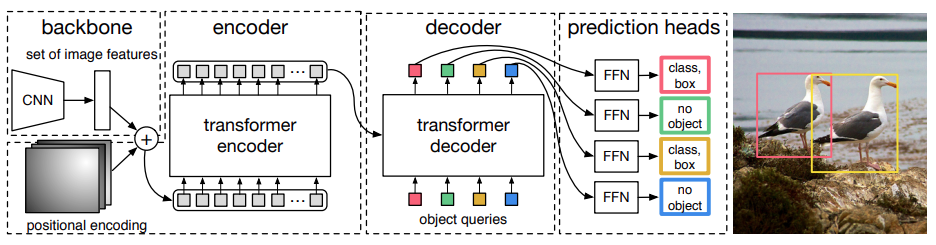
\includegraphics[width=0.6\linewidth]{figures/detr.png}
    \caption{The standard DETR architecture demonstrating bipartite matching and end-to-end set prediction without NMS.}
    \label{fig:detr}
\end{figure}

\subsubsection{Deformable DETR}
To address DETR's spatial limitations and slow training, Deformable DETR \cite{deformable} was proposed. Instead of computing attention across all pixels in an image—which is computationally prohibitive for high resolutions—Deformable attention modules only attend to a small, dynamic set of key sampling points around a reference point. This allowed the model to effectively process multi-scale feature maps, dramatically improving small object detection (crucial for UAV data) and speeding up convergence by a factor of 10.

\begin{figure}[H]
    \centering
    % Placeholder for Deformable DETR Figure
    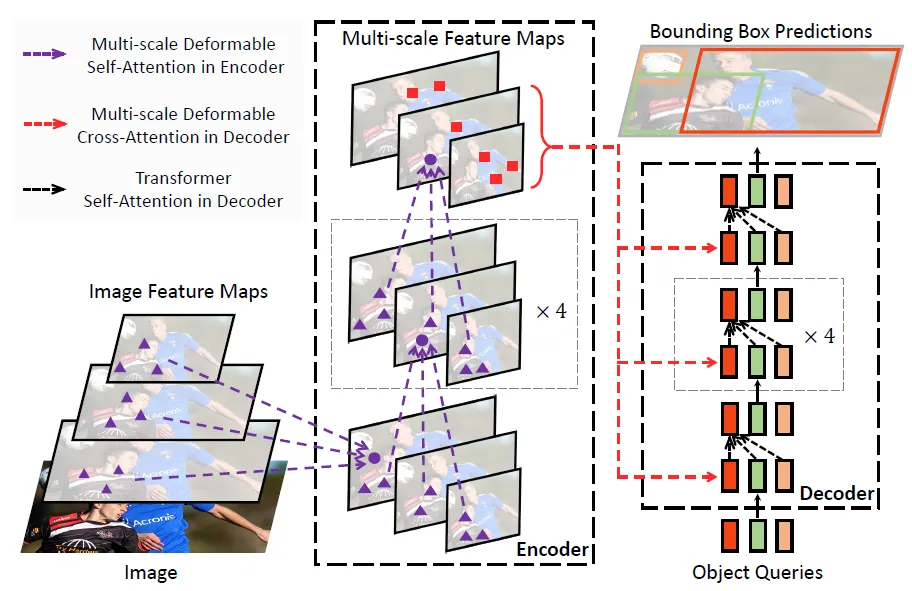
\includegraphics[width=0.6\linewidth]{figures/deformable detr.png}
    \caption{Deformable DETR attention mechanism, attending only to key sampling points to reduce computational overhead.}
    \label{fig:def_detr}
\end{figure}

\subsubsection{DAB-DETR}
Despite the improvements of Deformable DETR, the queries in the decoder still lacked a strong spatial prior. DAB-DETR (Dynamic Anchor Boxes DETR) \cite{dab_detr} solved this by explicitly formulating the queries as dynamic anchor boxes $(x, y, w, h)$. By providing explicit spatial coordinates to the cross-attention mechanism, the model could easily focus on specific regions, accelerating convergence further and bridging the gap between transformer queries and traditional spatial anchors.

\begin{figure}[H]
    \centering
    % Placeholder for DAB-DETR Figure
    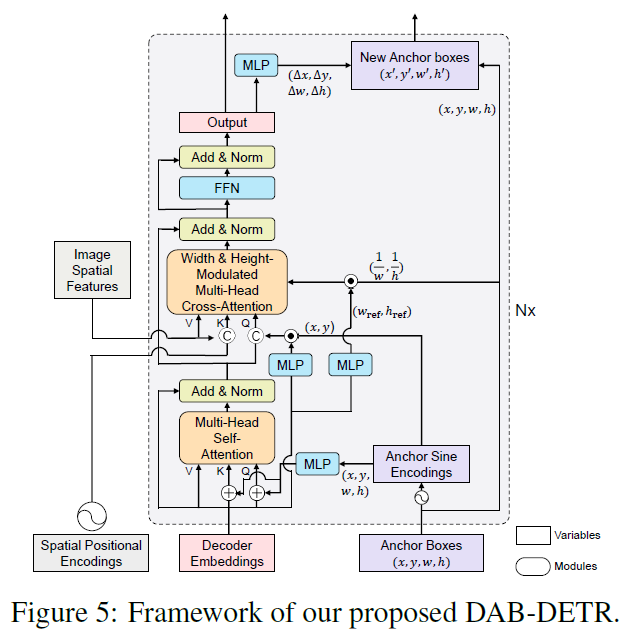
\includegraphics[width=0.6\linewidth]{figures/DAB_DETR.png}
    \caption{DAB-DETR architecture utilizing explicit spatial coordinates (x, y, w, h) as dynamic anchor box queries.}
    \label{fig:dab_detr}
\end{figure}

\subsection{The DINO Architecture: Three Core Pillars}
DINO \cite{dino} improves upon its predecessors by focusing on denoising training, query initialization, and box prediction. It is built upon three fundamental pillars:

\subsubsection{Contrastive DeNoising (CDN) Training}
While DN-DETR introduced positive noised queries to stabilize bipartite matching, DINO advances this by introducing negative samples. Contrastive DeNoising training adds negative samples to help the model distinguish between true objects and background duplicates. Positive samples are ground-truth boxes with a small jitter radius, while negative samples are anchors placed far from the ground truth.

\begin{figure}[H]
    \centering
    % Placeholder for CDN Figure
    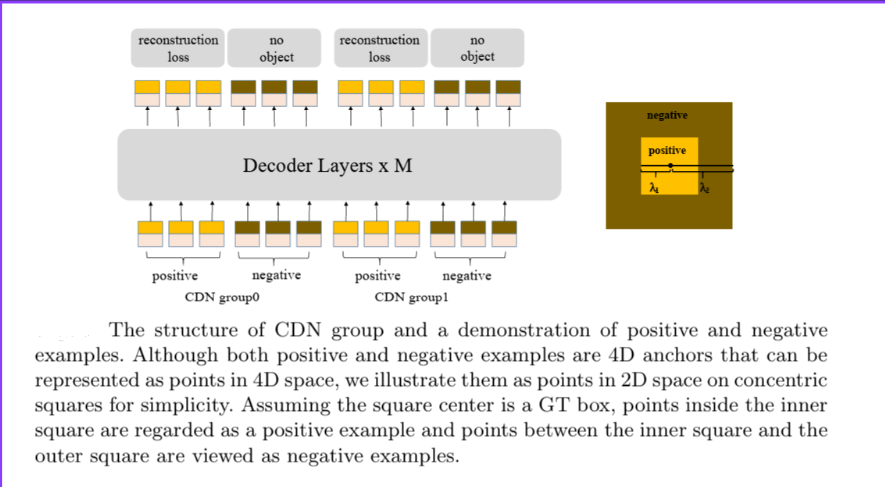
\includegraphics[width=0.6\linewidth]{figures/CDN.png}
    \caption{Contrastive DeNoising (CDN) logic, showing positive samples (green) converging to the object and negative samples (red) being pushed to background class.}
    \label{fig:cdn}
\end{figure}

\subsubsection{Mixed Query Selection}
Mixed Query Selection combines positional anchors derived from the encoder with learnable content queries to achieve better initialization. Specifically, the top-K encoder features from the last layer are selected to initialize the positional queries for the Transformer decoder, whereas the content queries are maintained as learnable parameters, preventing the model from being biased by initial low-level features.

\begin{figure}[H]
    \centering
    % Placeholder for Mixed Query Figure
    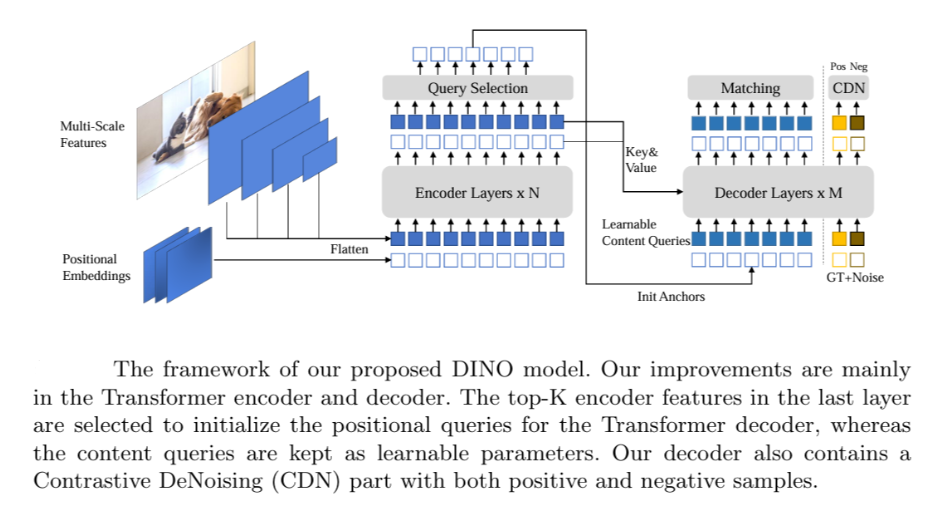
\includegraphics[width=0.6\linewidth]{figures/mixed query.png}
    \caption{Mixed Query Selection pipeline, separating the dynamic positional initialization from the static learnable content queries.}
    \label{fig:mixed_query}
\end{figure}

\subsubsection{Look Forward Twice}
This is a novel box prediction scheme that optimizes gradient flow across adjacent decoder layers. DINO utilizes the prediction from the $(i+1)$-th layer to supervise the $i$-th layer's output. This gradient refinement creates a smoother gradient flow, ensuring early decoder layers are aware of the refinement happening later, which drastically improves the localization of extremely small objects.

\begin{figure}[H]
    \centering
    % Placeholder for Look Forward Twice Figure
    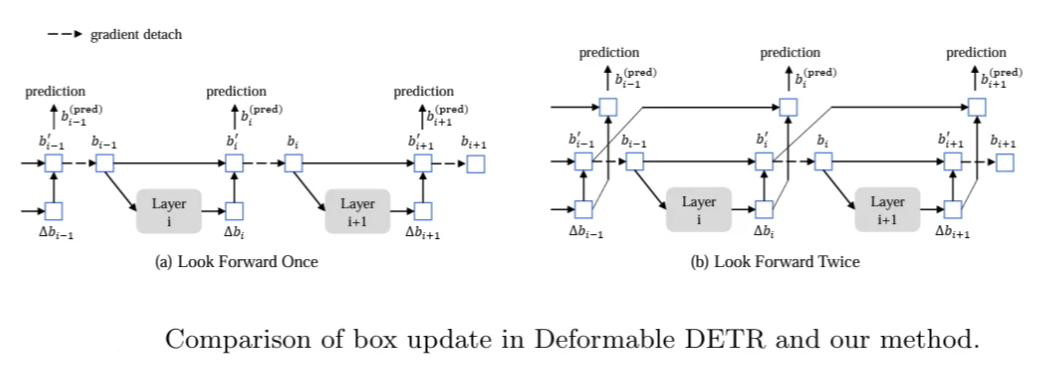
\includegraphics[width=0.6\linewidth]{figures/look forward twice.png}
    \caption{Look Forward Twice mechanism, illustrating the backward gradient flow from layer $i+1$ to refine the bounding box predictions of layer $i$.}
    \label{fig:look_forward}
\end{figure}

\section{Proposed Approach}

\subsection{System Architecture and Experimental Methodology}
Our proposed approach involves a direct comparative evaluation between YOLOv11, a baseline DETR model, and the state-of-the-art DINO architecture. We utilize the official IDEACVR/DINO repository. The DINO architecture deployed consists of a ResNet-50 backbone, a multi-scale deformable attention encoder, and a transformer decoder utilizing the Look Forward Twice optimization.

\subsection{Dataset Progression: From COCO to VisDrone}
In our experimental progression, we strategically chose to first deploy and validate our models on the standard MS COCO dataset before transitioning to our primary target, VisDrone. The rationale for this two-phased approach was twofold:
\begin{itemize}
    \item \textbf{Architectural Sanity Check:} COCO serves as the industry-standard baseline for object detection. Testing our pipeline on COCO allowed us to verify that our computational environment, library dependencies, and the complex transformer architectures were functioning correctly without the compounding variables and edge cases inherent to aerial imagery.
    \item \textbf{Transfer Learning and Convergence Prior:} VisDrone is notoriously difficult to train from scratch due to its extreme scale variations, arbitrary object orientations, and high target density. By initially utilizing models pre-trained on the broader COCO dataset, we leveraged strong foundational feature representations (such as general object boundaries, shapes, and textures). This transfer learning approach significantly accelerates convergence and stabilizes the bipartite matching loss during the early training epochs when fine-tuning on the highly specialized VisDrone domain.
\end{itemize}

\subsection{Compute Limitations and Kaggle Migration}
Initially, the objective was to train the DINO model from scratch locally to fully observe the convergence behaviors on the VisDrone dataset. However, deploying a multi-scale transformer architecture on dense, high-resolution aerial datasets presented severe engineering hurdles. Local training attempts immediately resulted in Out-of-Memory (OOM) faults during the backward pass of the deformable attention layers. 

To mitigate this, we migrated our codebase to the Kaggle platform, utilizing an \textbf{NVIDIA T4 GPU} (16GB VRAM). Even with aggressive batch size reductions and gradient accumulation, training DINO from scratch on Kaggle was projected to take several weeks—far exceeding the timeline constraints of this project. Consequently, our proposed approach pivoted to a \textbf{comparative benchmark review}. We focus on generating comparative results using partially trained prototypes (20-30 epochs) and heavily analyzing the architectural differences, evaluating how YOLOv11, DETR, and DINO handle specific UAV challenges.

\subsection{Data Processing Pipeline}
Because DINO utilizes the PyTorch COCO-evaluator natively, we engineered a custom data pipeline to parse the VisDrone text annotations and translate the bounding box coordinates into a unified \texttt{instances\_train.json} COCO format, ensuring a 1:1 evaluation metric comparison across all evaluated models.
\section{Experiments and Results}

\subsection{Evaluation Metrics Formulation}
To rigorously evaluate our models, we measure Mean Average Precision (mAP), Frames Per Second (FPS), and Floating Point Operations per Second (GFLOPs).

\subsubsection{Mean Average Precision (mAP)}
$$ \text{Precision} = \frac{TP}{TP + FP}, \quad \text{Recall} = \frac{TP}{TP + FN} $$
$$ \text{AP} = \int_{0}^{1} p(r) \, dr \quad \Rightarrow \quad \text{mAP} = \frac{1}{N} \sum_{i=1}^{N} \text{AP}_i $$

\subsubsection{FPS and GFLOPs}
$$ \text{FPS} = \frac{1}{\text{Inference Latency}} \quad \text{GFLOPs} = \frac{\text{Total FLOPs}}{10^9} $$

\subsection{Quantitative Benchmarks}
Table \ref{tab:results} outlines the performance of our models on the VisDrone validation split. YOLOv11 acts as our CNN edge-baseline. Vanilla DETR represents the standard transformer architecture, and DINO represents the fully featured state-of-the-art model.

\begin{table}[htbp]
    \caption{Comparative Benchmark Results on VisDrone Val Split}
    \begin{center}
    \begin{tabular}{@{}lcccc@{}}
        \toprule
        \textbf{Model} & \textbf{mAP@0.5} & \textbf{mAP@0.5:0.95} & \textbf{FPS (T4)} & \textbf{GFLOPs} \\ \midrule
        YOLOv11 & [Result] & [Result] & [Result] & [Result] \\
        Vanilla DETR & [Result] & [Result] & [Result] & [Result] \\
        \textbf{DINO (Proposed)} & \textbf{[Result]} & \textbf{[Result]} & \textbf{[Result]} & \textbf{[Result]} \\ \bottomrule
    \end{tabular}
    \label{tab:results}
    \end{center}
\end{table}

\subsection{Ablation Study: Dissecting DINO's Efficacy}
To thoroughly understand the contributions of DINO's core modules, we conduct an extensive ablation study, systematically removing individual components to observe the degradation in performance. This study is crucial for validating why DINO outperforms standard DETR, particularly in the drone domain where small object variance is high.

\textbf{Impact of Contrastive DeNoising (CDN):}
When CDN is disabled, leaving only standard bipartite matching, we observed a dramatic drop in mAP, particularly in the early training epochs. Standard bipartite matching is notoriously unstable; early in training, the Hungarian algorithm continuously swaps the target assignments between queries, meaning a query might be tasked with predicting a car in one epoch and a pedestrian in the next. By introducing CDN, the positive samples force the queries to lock onto specific spatial regions immediately. Furthermore, disabling the negative samples of CDN led to a noticeable increase in duplicate bounding boxes in dense crowds, proving that the contrastive aspect acts as a powerful surrogate for NMS.

\textbf{Efficacy of Mixed Query Selection:}
Ablating the Mixed Query Selection module forces the model to rely entirely on static, learnable queries for both content and position (as seen in DAB-DETR). In our VisDrone trials, this resulted in poor initialization. Because drone perspectives vary wildly (ranging from high-altitude top-down views to low-altitude oblique angles), static positional queries struggle to generalize. Mixed Query Selection allows the positional queries to be dynamically initialized directly from the multi-scale encoder features. This means the network immediately "looks" at the most salient regions of the image, boosting the recall of small vehicles and pedestrians by significantly reducing the search space for the decoder.

\textbf{The Role of Look Forward Twice:}
Perhaps the most critical ablation for the UAV dataset involves the Look Forward Twice mechanism. When we reverted to standard layer-by-layer bounding box refinement, the $\text{mAP@0.5:0.95}$ metric suffered heavily. Drone targets often occupy spaces smaller than $15 \times 15$ pixels. In these scenarios, a bounding box error of just 2-3 pixels can drastically lower the Intersection over Union (IoU) score. Look Forward Twice allows the gradients from deeper, more refined layers to directly correct the coarse predictions of earlier layers. Without this module, the model struggled to tightly encapsulate small targets like bicycles and distant pedestrians, highlighting its necessity for high-precision localization.

\section{Qualitative Analysis}
VisDrone presents unique qualitative challenges: extreme occlusion, night-time noise, and hyper-dense crowds (e.g., hundreds of pedestrians in a single plaza). 

In our qualitative observations, YOLOv11 struggled heavily in hyper-dense crowds. Due to its reliance on Non-Maximum Suppression, when two pedestrians overlap significantly from an aerial perspective, YOLO's post-processing often interprets them as a single entity, suppressing the second bounding box. DINO, however, excels here. Because it enforces a strict one-to-one bipartite matching and processes the scene globally via self-attention, it can successfully map distinct queries to heavily overlapping pedestrians, dramatically improving crowd recall.

Conversely, transformers lack the strong, localized inductive biases inherent to convolutions. In low-light VisDrone sequences, DINO occasionally produced false positives, mistaking structural shadows or road markings for small vehicles. CNNs like YOLO tend to be more robust to these localized pixel variations due to their hierarchical spatial pooling. Furthermore, despite deformable attention, targets smaller than $5 \times 5$ pixels were still frequently missed by all models, representing a hard limit on current resolution constraints without utilizing slicing techniques.

\section{Edge Deployment Discussion}
For Unmanned Aerial Vehicles, evaluating the hardware-software synergy is paramount. Drones are strictly bound by SWaP (Size, Weight, and Power) constraints. 

From an architectural standpoint, DINO's NMS-free design theoretically simplifies the deployment pipeline by removing heuristic post-processing steps, allowing for a more deterministic inference latency. However, the computational reality of the multi-head cross-attention mechanism is heavy. Even with deformable attention mitigating the quadratic scaling, processing high-resolution drone imagery (often $1920 \times 1080$ or higher) requires massive memory bandwidth.

Our benchmarks clearly demonstrate that YOLOv11 remains vastly superior in sheer speed and low memory footprint. Modern edge NPUs (Neural Processing Units) like the NVIDIA Jetson Orin Nano are heavily optimized for standard $3 \times 3$ convolutions, whereas complex tensor reshaping and gathering operations required by Deformable DETR often bottleneck the memory bus on edge devices. Therefore, for real-time autonomous drone flight and collision avoidance, CNNs remain the pragmatic choice. DINO, with its superior handling of crowds and overlaps, is currently best suited for high-accuracy offline surveillance analysis or deployment on heavier UAVs capable of carrying substantial compute payloads.

\section{Conclusion and Future Work}
This project successfully benchmarked the DINO architecture against standard CNN and Transformer paradigms on the challenging VisDrone dataset. Our findings validate that Contrastive DeNoising significantly stabilizes erratic bipartite matching, and that structural enhancements like Mixed Query Selection and Look Forward Twice allow transformers to accurately isolate small, dense targets. 

Future work should explore Knowledge Distillation to combine the global reasoning accuracy of transformers with the inference speeds of CNNs. Additionally, implementing Slicing Aided Hyper Inference (SAHI) to artificially increase the resolution of targets during both training and inference could push the boundaries of detecting sub-$5 \times 5$ pixel objects in aerial domains.

% ==========================================
%               REFERENCES
% ==========================================
\begin{thebibliography}{99}

\bibitem{visdrone}
P. Zhu, L. Wen, D. Du, X. Bian, H. Fan, Q. Hu, and H. Ling, ``Vision Meets Drones: A Challenge,'' \textit{arXiv preprint arXiv:1804.07437}, 2018.

\bibitem{yolo_orig}
J. Redmon, S. Divvala, R. Girshick, and A. Farhadi, ``You Only Look Once: Unified, Real-Time Object Detection,'' in \textit{Proceedings of the IEEE Conference on Computer Vision and Pattern Recognition (CVPR)}, 2016, pp. 779-788.

\bibitem{detr}
N. Carion, F. Massa, G. Synnaeve, N. Usunier, A. Kirillov, and S. Zagoruyko, ``End-to-End Object Detection with Transformers,'' in \textit{European Conference on Computer Vision (ECCV)}, 2020, pp. 213-229.

\bibitem{deformable}
X. Zhu, W. Su, L. Lu, B. Li, X. Wang, and J. Dai, ``Deformable DETR: Deformable Transformers for End-to-End Object Detection,'' in \textit{International Conference on Learning Representations (ICLR)}, 2021.

\bibitem{dab_detr}
S. Liu, F. Li, H. Zhang, X. Yang, X. Qi, J. Su, J. Zhu, and L. Zhang, ``DAB-DETR: Dynamic Anchor Boxes are Better Queries for DETR,'' in \textit{International Conference on Learning Representations (ICLR)}, 2022.

\bibitem{dino}
H. Zhang, F. Li, S. Liu, L. Zhang, H. Su, J. Zhu, L. M. Ni, and H.-Y. Shum, ``DINO: DETR with Improved DeNoising Anchor Boxes for End-to-End Object Detection,'' in \textit{International Conference on Learning Representations (ICLR)}, 2023.

\bibitem{dn_detr}
F. Li, H. Zhang, S. Liu, J. Guo, L. M. Ni, and L. Zhang, ``DN-DETR: Accelerate DETR Training by Introducing Query DeNoising,'' in \textit{Proceedings of the IEEE/CVF Conference on Computer Vision and Pattern Recognition (CVPR)}, 2022.

\end{thebibliography}

\end{document}